\documentclass[preprint,12pt,aps,pra,showkeys,amsmath,amssymb,superscriptaddress,floatfix]{revtex4-2}
\usepackage[T1]{fontenc}
\usepackage[utf8]{inputenc}
\usepackage{amsmath,amssymb,amsthm,mathtools,mathrsfs}
\usepackage{microtype,booktabs,enumitem}
\usepackage{xcolor,tikz,etoolbox}
\usepackage[skins,breakable]{tcolorbox}
\usepackage{needspace}
% Keep diagram geometry independent of REVTeX preprint body spacing.
\AtBeginEnvironment{tikzpicture}{\linespread{1}\selectfont}
\usetikzlibrary{arrows.meta,positioning,calc,fit,decorations.pathreplacing}
\usepackage{graphicx}
\usepackage{hyperref}

\definecolor{MMBlue}{RGB}{0,82,155}
\definecolor{MMOrange}{RGB}{200,80,0}
\tikzset{
 mmnode/.style={draw=MMBlue,rounded corners=2pt,fill=MMBlue!4,align=left,execute at begin node={\raggedright},text width=5cm,font=\fontsize{10}{12}\selectfont,inner sep=6pt},
 mmimport/.style={mmnode,draw=black!65,fill=black!4},
 mmcandidate/.style={mmnode,draw=MMOrange,dashed,fill=MMOrange!5},
 mmrejected/.style={mmnode,draw=black,densely dotted,fill=black!8},
 mmproof/.style={->,thick,MMBlue},
 mmflow/.style={->,semithick,black!70},
 mmrepair/.style={->,dashed,thick,MMOrange},
 mmcandidatearrow/.style={->,dashed,semithick,MMOrange},
 mmnote/.style={font=\scriptsize,fill=white,inner sep=2pt,align=center}}

\usepackage[section]{placeins}
\setlength{\emergencystretch}{3em}
\setlist{itemsep=3pt,topsep=4pt}
\newtheorem{theorem}{Theorem}[section]
\newtheorem{proposition}[theorem]{Proposition}
\newtheorem{lemma}[theorem]{Lemma}
\newtheorem{corollary}[theorem]{Corollary}
\theoremstyle{definition}
\newtheorem{definition}[theorem]{Definition}
\newtheorem{example}[theorem]{Example}
\theoremstyle{remark}
\newtheorem{remark}[theorem]{Remark}
% Avoid isolated statement headings and single-line paragraph fragments.
\BeforeBeginEnvironment{theorem}{\Needspace{6\baselineskip}}
\BeforeBeginEnvironment{definition}{\Needspace{5\baselineskip}}
\BeforeBeginEnvironment{proposition}{\Needspace{5\baselineskip}}
\BeforeBeginEnvironment{lemma}{\Needspace{5\baselineskip}}
\BeforeBeginEnvironment{corollary}{\Needspace{5\baselineskip}}
\clubpenalty=5000
\widowpenalty=5000
\newcommand{\R}{\mathbb R}\newcommand{\Z}{\mathbb Z}\newcommand{\N}{\mathbb N}
\newcommand{\Pa}{\operatorname{Pa}}\newcommand{\Desc}{\operatorname{Desc}}
\newcommand{\cl}{\operatorname{cl}}\newcommand{\cost}{\operatorname{cost}}
\newcommand{\status}{\operatorname{status}}
% Faculty cards: a visual rail groups the five faculties within one agent.
% The rail has no arrowhead and does not represent a proof dependency.
\newcommand{\mmfacultybadge}[1]{%
 \node[circle,draw=MMBlue,line width=1pt,fill=white,
 minimum size=7mm,inner sep=0pt,font=\sffamily\small\bfseries,text=MMBlue]
 at ([xshift=15pt,yshift=-15pt]frame.north west) {#1};}
\newcommand{\mmfacultyrail}{%
 \draw[MMBlue!80,line width=1pt]
 ([xshift=15pt,yshift=2pt]frame.north west)--
 ([xshift=15pt,yshift=-2pt]frame.south west);}
\newtcolorbox{mmfacultybox}[2]{enhanced,breakable,
 colback=MMBlue!4,colframe=MMBlue!4,boxrule=0pt,arc=3pt,
 left=39pt,right=9pt,top=4pt,bottom=4pt,
 before skip=2pt,after skip=2pt,
 fontupper=\small\linespread{1.1}\selectfont,
 overlay unbroken={\mmfacultyrail\mmfacultybadge{#1}},
 overlay first={\mmfacultyrail\mmfacultybadge{#1}},
 overlay middle={\mmfacultyrail},overlay last={\mmfacultyrail}}
\newcommand{\mmfaculty}[3]{%
 \begin{mmfacultybox}{#1}{#2}
 {\sffamily\bfseries\color{MMBlue}#2}\par\smallskip #3
 \end{mmfacultybox}}
\newcommand{\agent}[9]{%
 \Needspace{8\baselineskip}
 \subsubsection{#1}
 \noindent\textbf{Object.} #2\par
 \noindent\textbf{Role.} #3\par\smallskip
 \mmfaculty{E}{Ego}{#4}
 \mmfaculty{M}{Memory}{#5}
 \mmfaculty{I}{Intellect}{#6}
 \mmfaculty{S}{Sense}{#7}
 \mmfaculty{A}{Action}{#8}
 \smallskip\noindent #9\par}

\usepackage{longtable,array,calc}
\providecommand{\tightlist}{\setlength{\itemsep}{2pt}\setlength{\parskip}{0pt}}
\makeatletter
\def\frontmatter@abstract@produce{\par\addvspace{\frontmatter@preabstractspace}%
\begingroup\prep@absbox\unvbox\absbox\post@absbox\endgroup
\addvspace{\frontmatter@postabstractspace}}
\makeatother
\newcommand{\field}[2]{\par\smallskip\noindent\textbf{#1.} #2\par}
\setlength{\emergencystretch}{5em}
\AtBeginEnvironment{verbatim}{\small\linespread{1.0}\selectfont}


\hypersetup{colorlinks=true,linkcolor=MMBlue,urlcolor=MMBlue,pdfauthor={Dibakar Sigdel}}

\begin{document}

\title{Arzelà--Ascoli Theorem\\[4pt]\large An End-to-End Meta-Math Walkthrough}

\author{Dibakar Sigdel}

\affiliation{Mindverse Computing LLC, Lynnwood, WA 98087, USA}

\date{October 2026}

\begin{abstract}

A complete authored walkthrough of arzelà--ascoli theorem, with explicit
mathematical contracts, local verification gates, and reusable exports.
The report presents the target theorem, declared imports, a dependency
graph, five-faculty node contracts, a continuous proof, a worked
example, and a hypothesis-repair audit. It is an authored mathematical
exposition, not a deployed-agent transcript or a formal proof-assistant
certificate.

\end{abstract}\maketitle\linespread{1.12}\selectfont

\noindent\textbf{RA-05 / Real Analysis / Report v1}

\section{Target and import contract}

\begin{theorem}

For compact metric \(K\), prove that
\(\mathcal F\subset C(K,\mathbb R)\) is relatively compact in the
supremum norm if and only if it is uniformly bounded and equicontinuous.

\end{theorem}

\subsection{Foundations and permitted imports}

For compact metric K, finite \(\varepsilon\)-nets exist.
Bolzano--Weierstrass applies to bounded real sequences. \(C(K)\) with
supremum norm is complete; a uniform limit of continuous functions is
continuous. In metric spaces compactness equals sequential compactness,
and complete totally bounded spaces are compact. These elementary metric
lemmas are permitted imports.

\clearpage\section{Node interaction workflow}

\begin{center}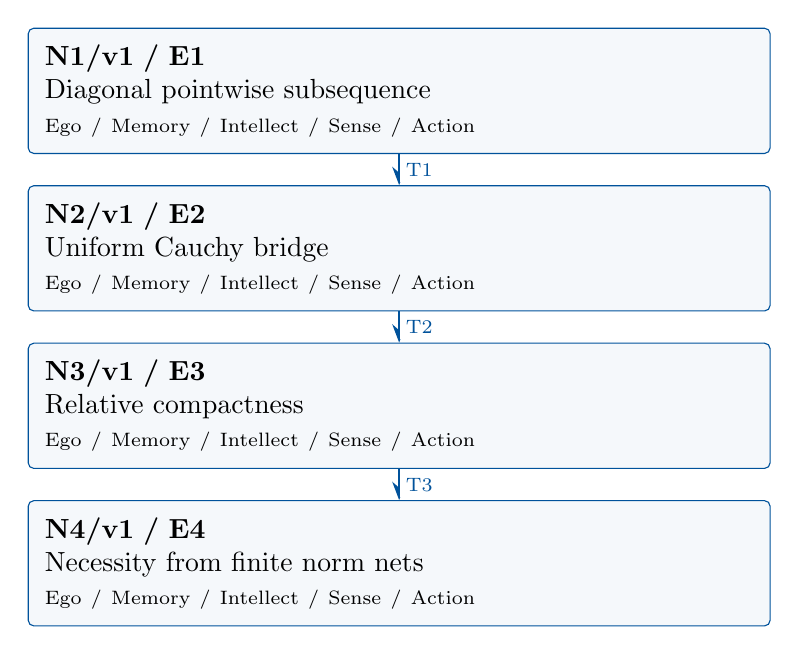
\begin{tikzpicture}[>=Stealth,x=1cm,y=1cm]

\node[mmnode,text width=9cm,minimum height=1.25cm] (N1) at (0,0.0) {\textbf{N1/v1 / E1}\\Diagonal pointwise subsequence\\{\scriptsize Ego / Memory / Intellect / Sense / Action}};

\node[mmnode,text width=9cm,minimum height=1.25cm] (N2) at (0,-2.0) {\textbf{N2/v1 / E2}\\Uniform Cauchy bridge\\{\scriptsize Ego / Memory / Intellect / Sense / Action}};

\node[mmnode,text width=9cm,minimum height=1.25cm] (N3) at (0,-4.0) {\textbf{N3/v1 / E3}\\Relative compactness\\{\scriptsize Ego / Memory / Intellect / Sense / Action}};

\node[mmnode,text width=9cm,minimum height=1.25cm] (N4) at (0,-6.0) {\textbf{N4/v1 / E4}\\Necessity from finite norm nets\\{\scriptsize Ego / Memory / Intellect / Sense / Action}};

\draw[mmproof] (N1.south) -- node[mmnote,right] {T1} (N2.north);

\draw[mmproof] (N2.south) -- node[mmnote,right] {T2} (N3.north);

\draw[mmproof] (N3.south) -- node[mmnote,right] {T3} (N4.north);

\end{tikzpicture}\end{center}

Each box is one mathematical agent containing all five faculties. Blue
arrows carry the versioned exports listed below. The layout gives a
reading order; only drawn arrows assert dependencies. Diagnostic repair
is separate from the proof DAG.

\clearpage\subsection{Versioned evidence-transfer ledger}

\begingroup\small\linespread{1.05}\selectfont

\Needspace{5\baselineskip}\field{T1: N1/E1/v1 to N2}{A subsequence converges at all points of a countable dense set.}

\field{Receiving activity}{N2: Uniform Cauchy bridge}

\field{Compatibility}{Use the same mathematical objects and hypotheses as the source export.
Receiving contract: Diagonal convergence; uniform equicontinuity; prior
exports E1/v1}

\Needspace{5\baselineskip}\field{T2: N2/E2/v1 to N3}{Every sequence in F has a uniformly convergent subsequence in \(C(K)\).}

\field{Receiving activity}{N3: Relative compactness}

\field{Compatibility}{Use the same mathematical objects and hypotheses as the source export.
Receiving contract: Subsequence property; prior exports E2/v1}

\Needspace{5\baselineskip}\field{T3: N3/E3/v1 to N4}{Uniform boundedness and equicontinuity imply relative compactness.}

\field{Receiving activity}{N4: Necessity from finite norm nets}

\field{Compatibility}{Use the same mathematical objects and hypotheses as the source export.
Receiving contract: Compact \(\operatorname{closure} (F)\); prior export
E3/v1 for the final equivalence synthesis}

\endgroup

\clearpage\section{Agent roles and five-faculty activities}\begingroup\small\linespread{1.05}\selectfont\setlist{itemsep=1pt,topsep=2pt}

\subsection{N1/v1: Diagonal pointwise subsequence}

\field{Object and role}{Exploit a countable dense set supplied by finite nets.}

\field{Inputs}{Uniform boundedness and equicontinuity of F; foundational imports stated
in §1}

\mmfaculty{E}{Ego}{Own E1/v1: A subsequence converges at all points of a countable dense
set.}

\mmfaculty{M}{Memory}{Retain Uniform boundedness and equicontinuity of F; foundational imports
stated in §1; keep their assumptions and versions attached.}

\mmfaculty{I}{Intellect}{Exploit a countable dense set supplied by finite nets.}

\mmfaculty{S}{Sense}{A dense set alone does not imply uniform convergence.}

\mmfaculty{A}{Action}{Carry out the numbered deductions and publish E1/v1 together with its
hypotheses and proof location.}

\smallskip\noindent\textbf{Numbered mathematical activities}

\begin{enumerate}[label=N1.\arabic*,leftmargin=3.4em]

\item Assume K nonempty; if it is empty the function space has one element.

\item Unite finite1/j-nets to obtain a countable dense
\(set\{z_{1},z_{2},\ldots \}\).

\item Given any sequence in F, repeatedly extract subsequences converging at
\(z_j\) using boundedness and Bolzano--Weierstrass.

\item The diagonal subsequence \(g_j\) converges at every fixed \(z_i\).

\end{enumerate}

\field{Export E1/v1}{A subsequence converges at all points of a countable dense set.}

\field{Acceptance gate}{A dense set alone does not imply uniform convergence. Publish only after
checking every displayed deduction.}

\field{Targeted repair}{If the check fails, revise N1: A dense set alone does not imply uniform
convergence. Recheck dependent nodes N2, N3, N4.}

\clearpage

\subsection{N2/v1: Uniform Cauchy bridge}

\field{Object and role}{Control the entire space by finitely many nearby sampled points.}

\field{Inputs}{Diagonal convergence; uniform equicontinuity; prior exports E1/v1}

\mmfaculty{E}{Ego}{Own E2/v1: Every sequence in F has a uniformly convergent subsequence in
\(C(K)\).}

\mmfaculty{M}{Memory}{Retain Diagonal convergence; uniform equicontinuity; prior exports
E1/v1; keep their assumptions and versions attached.}

\mmfaculty{I}{Intellect}{Control the entire space by finitely many nearby sampled points.}

\mmfaculty{S}{Sense}{The \(\delta\) is common to the family, not chosen separately for each
function.}

\mmfaculty{A}{Action}{Carry out the numbered deductions and publish E2/v1 together with its
hypotheses and proof location.}

\smallskip\noindent\textbf{Numbered mathematical activities}

\begin{enumerate}[label=N2.\arabic*,leftmargin=3.4em]

\item Given \(\varepsilon >0\) choose \(\delta\) so \(d(x,y)<\delta\) implies
\(|h(x)-h(y)|<\varepsilon /3\) for every \(h\in F\).

\item Choose a finite \(\delta\)-net whose centers lie in the dense set.

\item For large j,k all finitely many center differences
\(|g_j(z_i)-g_k(z_i)|\) are below \(\varepsilon /3\).

\item For arbitrary x choose a center within \(\delta\); the triangle
inequality gives \(|g_j(x)-g_k(x)|<\varepsilon\).

\item Completeness of \(C(K)\) supplies a uniform continuous limit.

\item Every sequence in F has such a subsequence.

\end{enumerate}

\field{Export E2/v1}{Every sequence in F has a uniformly convergent subsequence in \(C(K)\).}

\field{Acceptance gate}{The \(\delta\) is common to the family, not chosen separately for each
function. Publish only after checking every displayed deduction.}

\field{Targeted repair}{If the check fails, revise N2: The \(\delta\) is common to the family,
not chosen separately for each function. Recheck dependent nodes N3, N4.}

\clearpage

\subsection{N3/v1: Relative compactness}

\field{Object and role}{Extend the property to the closure.}

\field{Inputs}{Subsequence property; prior exports E2/v1}

\mmfaculty{E}{Ego}{Own E3/v1: Uniform boundedness and equicontinuity imply relative
compactness.}

\mmfaculty{M}{Memory}{Retain Subsequence property; prior exports E2/v1; keep their assumptions
and versions attached.}

\mmfaculty{I}{Intellect}{Extend the property to the closure.}

\mmfaculty{S}{Sense}{A limit need not belong to F itself, only its closure.}

\mmfaculty{A}{Action}{Carry out the numbered deductions and publish E3/v1 together with its
hypotheses and proof location.}

\smallskip\noindent\textbf{Numbered mathematical activities}

\begin{enumerate}[label=N3.\arabic*,leftmargin=3.4em]

\item For a sequence \(h_j\) in the closure of F choose \(g_j\in F\) with
\(\Vert h_j-g_j\Vert \infty <1/j\).

\item A uniformly convergent subsequence of \(g_j\) forces the corresponding
\(h_j\) to converge to the same limit, which lies in the closed set
\(\operatorname{closure} (F)\).

\item Its closure is therefore sequentially compact and hence compact by the
metric lemma.

\item This proves sufficiency.

\end{enumerate}

\field{Export E3/v1}{Uniform boundedness and equicontinuity imply relative compactness.}

\field{Acceptance gate}{A limit need not belong to F itself, only its closure. Publish only
after checking every displayed deduction.}

\field{Targeted repair}{If the check fails, revise N3: A limit need not belong to F itself, only
its closure. Recheck dependent nodes N4.}

\clearpage

\subsection{N4/v1: Necessity from finite norm nets}

\field{Object and role}{Turn compactness into uniform bounds and a shared continuity modulus.}

\field{Inputs}{Compact \(\operatorname{closure} (F)\); prior export E3/v1 for the final
equivalence synthesis}

\mmfaculty{E}{Ego}{Own E4/v1: Relative compactness is equivalent to both stated family
conditions.}

\mmfaculty{M}{Memory}{Retain Compact \(\operatorname{closure} (F)\); prior export E3/v1 for
the final equivalence synthesis; keep their assumptions and versions
attached.}

\mmfaculty{I}{Intellect}{Turn compactness into uniform bounds and a shared continuity modulus.}

\mmfaculty{S}{Sense}{Pointwise boundedness is not the hypothesis used in the diagonal step
unless compact equicontinuity is separately used to upgrade it.}

\mmfaculty{A}{Action}{Carry out the numbered deductions and publish E4/v1 together with its
hypotheses and proof location.}

\smallskip\noindent\textbf{Numbered mathematical activities}

\begin{enumerate}[label=N4.\arabic*,leftmargin=3.4em]

\item Cover \(\operatorname{closure} (F)\) by finitely many norm balls of
radius 1 centered at \(h_i\).

\item Then
\(\Vert f\Vert \infty \le 1+\operatorname{max} _i\Vert h_i\Vert \infty\).

\item For \(\varepsilon >0\) choose a finite norm net of radius
\(\varepsilon /3\) with continuous centers \(h_i\).

\item Each center is uniformly continuous on K; choose one \(\delta\) valid
for all finitely many.

\item For \(d(x,y)<\delta\) and f within \(\varepsilon /3\) of \(h_i\),
\(|f(x)-f(y)|\le 2\Vert f-h_i\Vert \infty +|h_i(x)-h_i(y)|<\varepsilon\).

\item Thus F is equicontinuous; both directions close.

\end{enumerate}

\field{Export E4/v1}{Relative compactness is equivalent to both stated family conditions.}

\field{Acceptance gate}{Pointwise boundedness is not the hypothesis used in the diagonal step
unless compact equicontinuity is separately used to upgrade it. Publish
only after checking every displayed deduction.}

\field{Targeted repair}{If the check fails, revise N4: Pointwise boundedness is not the
hypothesis used in the diagonal step unless compact equicontinuity is
separately used to upgrade it. Withhold this terminal result until its
gate passes.}

\endgroup\clearpage\section{Continuous mathematical proof}\label{sec:proof}

Read these steps in order as one proof; the diagram is optional.
Numbered activities identify the specific constructions and deductions
owned by each node.

\subsection{§4.N1 --- Diagonal pointwise
subsequence}\label{n1-diagonal-pointwise-subsequence}

\begin{enumerate}
\def\labelenumi{\arabic{enumi}.}
\item
  Assume K nonempty; if it is empty the function space has one element.
\item
  Unite finite1/j-nets to obtain a countable dense
  \(set\{z_{1},z_{2},\ldots \}\).
\item
  Given any sequence in F, repeatedly extract subsequences converging at
  \(z_j\) using boundedness and Bolzano--Weierstrass.
\item
  The diagonal subsequence \(g_j\) converges at every fixed \(z_i\).
\end{enumerate}

\subsection{§4.N2 --- Uniform Cauchy
bridge}\label{n2-uniform-cauchy-bridge}

\begin{enumerate}
\def\labelenumi{\arabic{enumi}.}
\item
  Given \(\varepsilon >0\) choose \(\delta\) so \(d(x,y)<\delta\)
  implies \(|h(x)-h(y)|<\varepsilon /3\) for every \(h\in F\).
\item
  Choose a finite \(\delta\)-net whose centers lie in the dense set.
\item
  For large j,k all finitely many center differences
  \(|g_j(z_i)-g_k(z_i)|\) are below \(\varepsilon /3\).
\item
  For arbitrary x choose a center within \(\delta\); the triangle
  inequality gives \(|g_j(x)-g_k(x)|<\varepsilon\).
\item
  Completeness of \(C(K)\) supplies a uniform continuous limit.
\item
  Every sequence in F has such a subsequence.
\end{enumerate}

\subsection{§4.N3 --- Relative
compactness}\label{n3-relative-compactness}

\begin{enumerate}
\def\labelenumi{\arabic{enumi}.}
\item
  For a sequence \(h_j\) in the closure of F choose \(g_j\in F\) with
  \(\Vert h_j-g_j\Vert \infty <1/j\).
\item
  A uniformly convergent subsequence of \(g_j\) forces the corresponding
  \(h_j\) to converge to the same limit, which lies in the closed set
  \(\operatorname{closure} (F)\).
\item
  Its closure is therefore sequentially compact and hence compact by the
  metric lemma.
\item
  This proves sufficiency.
\end{enumerate}

\subsection{§4.N4 --- Necessity from finite norm
nets}\label{n4-necessity-from-finite-norm-nets}

\begin{enumerate}
\def\labelenumi{\arabic{enumi}.}
\item
  Cover \(\operatorname{closure} (F)\) by finitely many norm balls of
  radius 1 centered at \(h_i\).
\item
  Then
  \(\Vert f\Vert \infty \le 1+\operatorname{max} _i\Vert h_i\Vert \infty\).
\item
  For \(\varepsilon >0\) choose a finite norm net of radius
  \(\varepsilon /3\) with continuous centers \(h_i\).
\item
  Each center is uniformly continuous on K; choose one \(\delta\) valid
  for all finitely many.
\item
  For \(d(x,y)<\delta\) and f within \(\varepsilon /3\) of \(h_i\),
  \(|f(x)-f(y)|\le 2\Vert f-h_i\Vert \infty +|h_i(x)-h_i(y)|<\varepsilon\).
\item
  Thus F is equicontinuous; both directions close.
\end{enumerate}

\hfill$\square$

\section{Worked orchestration}

The functions on{[}0,1{]} with \(|f|\le 1\) and Lipschitz constant
\(\le 1\) are equicontinuous, so every sequence has a uniform convergent
subsequence. The proof takes common \(\delta =\varepsilon /3\) and
finitely many rational grid centers; the limit keeps the same bounds.

\subsection{Boundary and hypothesis audit}

The family \(x\mapsto x^{n}\) on{[}0,1{]} is uniformly bounded but not
equicontinuous at 1. Its only possible pointwise limit has a jump at 1,
so no subsequence converges uniformly. Sense rejects treating
boundedness as sufficient and routes the failure to the common-modulus
node.

\section{Illustrative failure and repair}

The following is an authored diagnostic scenario. Changed assumptions
define a new contract; they do not retroactively prove the original
statement.

\subsection{Failure and correction}
This is an authored teaching trace, not a recorded agent run.

\begin{enumerate}
\def\labelenumi{\arabic{enumi}.}
\tightlist
\item
  \textbf{Ego \(\to\) Memory:} register the §1 theorem, imports, and
  requested exports before beginning the proof.
\item
  \textbf{Intellect \(\to\) Action:} choose the bridges in §3 and carry
  out the numbered activities in §4; transmit only established E-exports
  along the §2 DAG.
\item
  \textbf{Sense \(\to\) responsible node:} test the specific
  boundary/failure in §5 and the node's individual audit. A failing
  candidate is withheld; downstream nodes may not use it.
\item
  \textbf{Memory + Intellect:} identify whether the error is an omitted
  condition, an invalid inference, or an attempted extension beyond the
  theorem. Restore the exact contract or explicitly state a different
  one.
\item
  \textbf{Action:} redo the affected mathematical activity using the
  repaired condition or inference. Recheck consuming nodes, rather than
  feeding their conclusions back as premises.
\item
  \textbf{Ego:} publish only the supported export with its assumptions
  and proof location. A hypothetical revised export is v2; the written
  proof here is the v1 exposition, not a claim that this repair was
  executed.
\end{enumerate}

\subsection{Hypothesis boundary}
The family \(x\mapsto x^{n}\) on{[}0,1{]} is uniformly bounded but not
equicontinuous at 1. Its only possible pointwise limit has a jump at 1,
so no subsequence converges uniformly. Sense rejects treating
boundedness as sufficient and routes the failure to the common-modulus
node.

\subsection{Version and recheck}
Treat any changed assumption as a new contract. Recheck the revised
export and all of its descendants. A backward diagnostic never
establishes an earlier theorem. This is an authored teaching trace, not
an execution log.

\par\medskip\begingroup\small\linespread{1.0}\selectfont\noindent\textbf{Provenance.} This authored proof is complete relative to its declared imports. Reuse
each export with its assumptions, proof, and version. The original
Markdown remains available for comparison.
\par\endgroup

\end{document}
